% Generated by thesis/ch7/exp2/networks.py -- do not edit by hand.
\begin{sidewaysfigure}
  \centering
  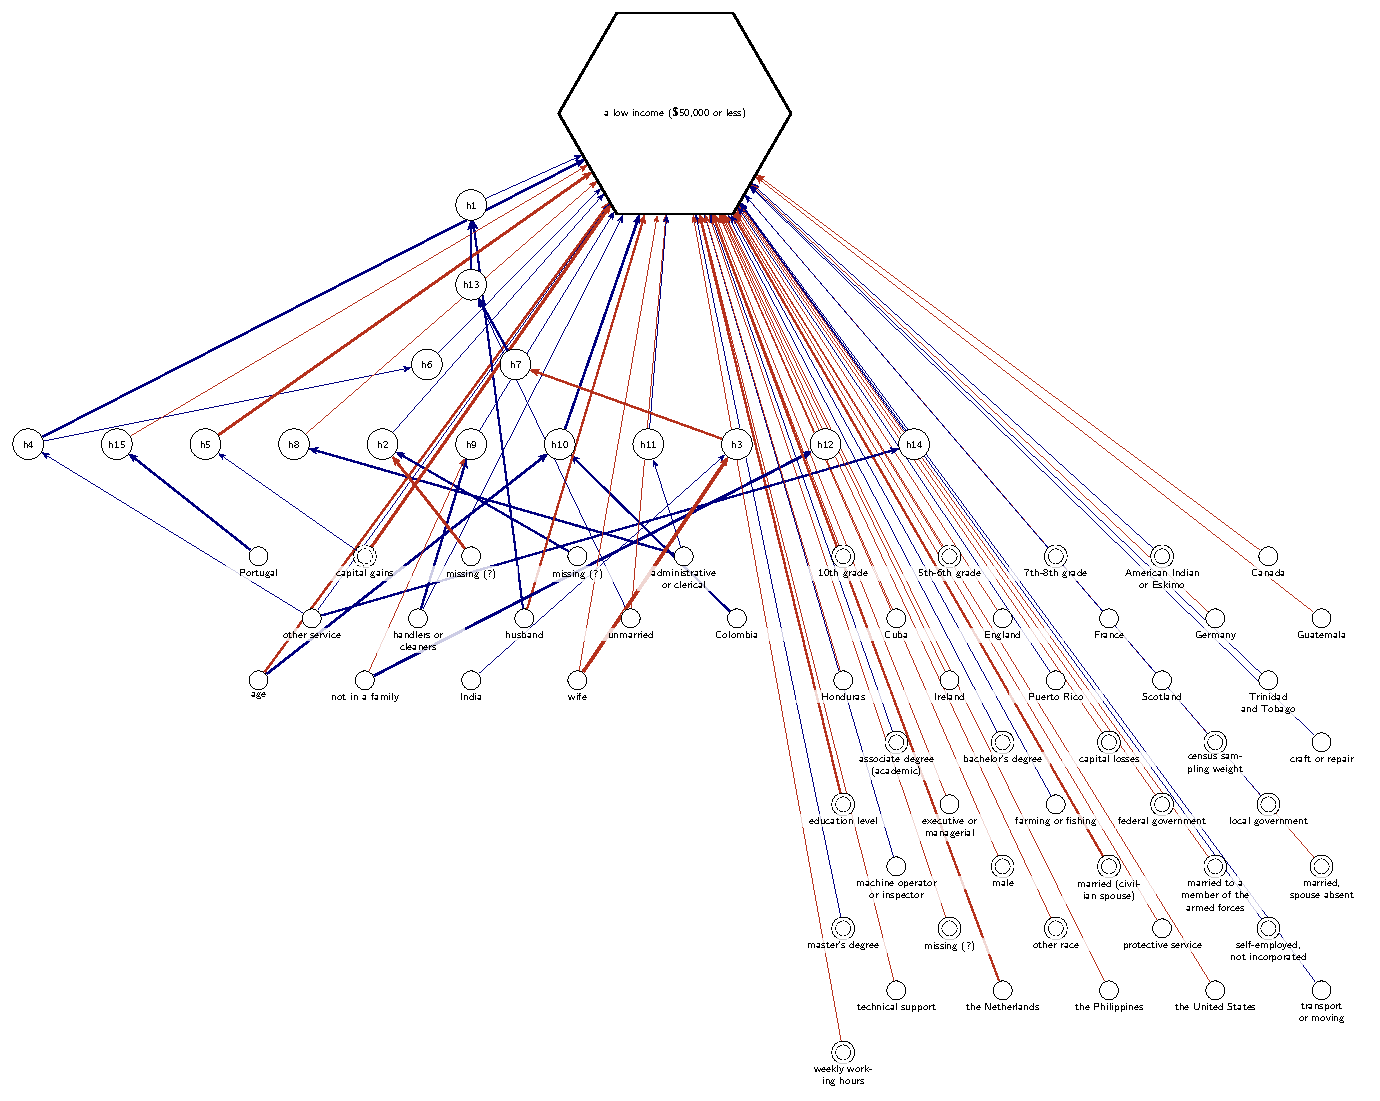
\includegraphics[width=\textheight,height=0.78\textwidth,keepaspectratio]{figures/exp2/networks/adult-s4-raw}
  \caption{Adult, seed 4 (adult-s4): the network as trained, before any explanation, in full. Inputs at the bottom (every input column its own node), hidden units by depth, the output at the top; 55 of 107 input columns are connected, with 15 hidden units and 81 enabled connections. Blue: positive weight (raises the score); red: negative weight (lowers it); thicker: larger weight. Orange outline and up arrow: raises the final prediction; teal and down arrow: lowers it; grey and double arrow: depends. Not used (no connection; 52 columns): never worked, private, self-employed, incorporated, state government, without pay, 11th grade, doctorate, high-school graduate, preschool, professional school degree, some college, 12th grade (no diploma), 1st-4th grade, 9th grade, associate degree (vocational), divorced, never married, separated, widowed, professional specialty, sales, armed forces, private household service, other relative, own child, Asian or Pacific Islander, Black, White, Cambodia, Greece, Haiti, Hong Kong, Hungary, Iran, Italy, Jamaica, Japan, Laos, Mexico, Nicaragua, outlying US territories (Guam, US Virgin Islands), Peru, China, Poland, 'South' (as recorded), Taiwan, Thailand, Vietnam, Yugoslavia, Dominican Republic, Ecuador and El Salvador.}
  \label{fig:exp2-net-adult-s4-raw}
\end{sidewaysfigure}
